% Chapter 1

\chapter{Introduction} % Main chapter title

\label{Chapter1} % For referencing the chapter elsewhere, use \ref{Chapter1}

%----------------------------------------------------------------------------------------

% Define some commands to keep the formatting separated from the content
\newcommand{\keyword}[1]{\textbf{#1}}
\newcommand{\tabhead}[1]{\textbf{#1}}
\newcommand{\code}[1]{\texttt{#1}}
\newcommand{\file}[1]{\texttt{\bfseries#1}}
\newcommand{\option}[1]{\texttt{\itshape#1}}

%********************************** %First Section  **************************************
\section{Background} %Section - 1.1

This article describes the design of a small or medium-sized library management system. Focusing on the technical perspective, the planning of the small and medium-sized library database management system and the design of the main function modules are discussed.
The libraries described in this article are not the same as the public library, but also different from the higher school library. The main manifestations are:
(1) From the perspective of the book star, it belongs to the small and medium-sized (generally in the tens of thousands of volumes). Due to the limited funds, the distribution of the types of books is closely related to the professional settings of the institutions.
(2) The number of readers is limited (generally around a thousand people), and the time rules for book retrieval and borrowing are strong. ( ) 3 There are fewer library staff, which makes the professional division of labor less clear, and often one person has several positions.
In order to improve the quality of the book collection, use the limited collection of books more effectively, provide readers with high-quality services, and make the management of the library scientific and modern, we have developed a library database system on the microcomputer, system development. Fully consider the characteristics of the secondary professional school library, and strive to make it have the management functions of small and medium-sized libraries.
This Library management system requires the ability to divide and set the features and permissions of books, readers, system administrators and other roles. The system is required to operate correctly and the operation interface is simple and easy to understand.


%********************************** %Second Section  *************************************
\section{System's Objective} %Section - 1.2

The main functions of the system are: it can manage the system user information and permissions, can manage the book information, can manage the reader information, can carry out the book borrowing operation and record the borrowing information. After the group discussion, the system should mainly have the following Features:

\begin{itemize}
    \item \textbf{Features One:} Modify book information, manage system administrators and set up all departments, manage bookshelf number and save books, exit system;
    \item \textbf{Features Two:} Manage reader information and types, new users can register themselves, administrators have the permission to add or delete users;
    \item \textbf{Features Three:} Borrow books, return books, check loan's status;
    \item \textbf{Featrues Four:} Add "Groups", to let readers with similar interests discuss in the same group; administrators can create new groups, users can join groups
\end{itemize}

\section{Introduction to system flow}

\begin{figure}[htbp!]
\centering
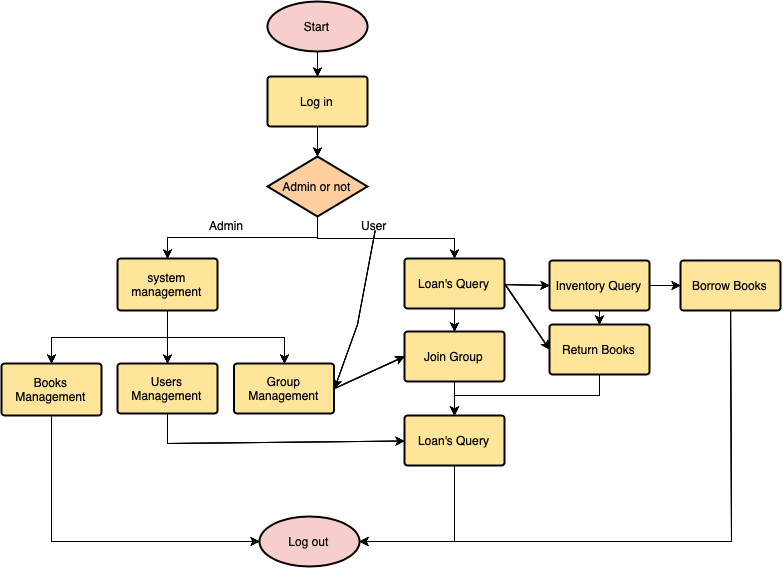
\includegraphics[width=1.0\textwidth]{Figures/Flowchart.png}
\caption[Figures/origindata.png]{Flowchart}
\label{fig:System Flow Chart}
\end{figure}
